\section{Failed Attempt}
\begin{leftbar}
    \noindent
    At first, it was attempted to create a custom algorithm capable of streamline placement in 3D.
    We then wanted to introduce changes that allowed the lines to be placed adhering to spatial coherence.
    Unfortunately, this was met with failure relatively quickly.
    The algorithm proposed was simply too greedy, and did not yield good initial results.
    Adding time coherence in this case would be of very little benefit here, since the initial image quality and performance degraded way too quickly for it to be actually useful.
    We still outline some of it in this chapter, in case it is of interest or as an example.
\end{leftbar}
\noindent
We start with a simple algorithm to generate streamlines in a 2D slice of a vector field.
The local z-component of the Cartesian grid is simply set to zero for the relevant sections of the algorithm.
The algorithm uses two operations: Streamline Traversal and Seed Filtering, which are executed round-robin.
\subsection{Streamline Traversal}
The Streamline Traversal process works as follows:
\begin{itemize}
    \begin{minipage}{.6\textwidth}
    \item \textbf{Step 1:}
    Choose a seed point from a list of candidates (initially an arbitrary point from the dataset) and remove it from the list.
    Then integrate forward and backward to obtain the other points on the streamline, until
    a number of steps is reached, we cross the bounding box, or we get too close to another streamline.
    \item \textbf{Step 2:}
    Compute the normals, add and subtract them to the succeeding point. The first point (according to step count in backward iteration) will not have a preceding normal, and is not used in this step. These points are new seed candidates for further streamline placement.
    \end{minipage}
    \begin{minipage}{.3\textwidth}
    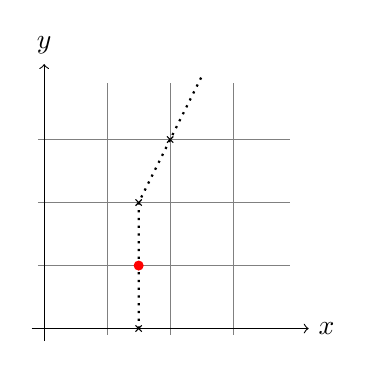
\begin{tikzpicture}[domain=0:4, scale=.8]
    \draw[very thin,color=gray] (-0.1,-0.1) grid (3.9,3.9);

    \draw[->] (-0.2,0) -- (4.2,0) node[right] {$x$};
    \draw[->] (0,-0.2) -- (0,4.2) node[above] {$y$};

    \draw[dotted, thick] (1.5,0) -- (1.5,2) -- (2.5,4);

    \draw[red] plot[only marks, mark=*] coordinates{(1.5,1)};
    \draw plot[only marks, mark=x] coordinates{(1.5,0) (1.5,2) (2,3)};
\end{tikzpicture}

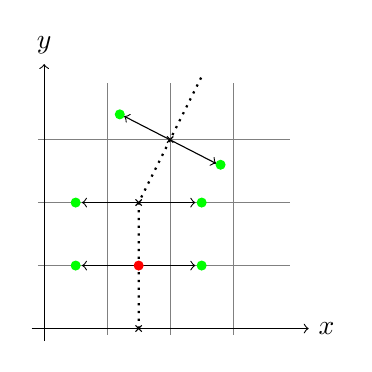
\begin{tikzpicture}[domain=0:4, scale=.8]
    \draw[very thin,color=gray] (-0.1,-0.1) grid (3.9,3.9);
    
    \draw[->] (-0.2,0) -- (4.2,0) node[right] {$x$};
    \draw[->] (0,-0.2) -- (0,4.2) node[above] {$y$};

    \draw[<->] (0.6, 1) -- (2.4, 1);
    \draw[<->] (0.6, 2) -- (2.4, 2);
    \draw[<->] (1.27, 3.37) -- (2.73, 2.62);
    
    \draw[dotted, thick] (1.5,0) -- (1.5,2) -- (2.5,4);
    
    \draw[red] plot[only marks, mark=*] coordinates{(1.5,1)};
    \draw plot[only marks, mark=x] coordinates{(1.5,0) (1.5,2) (2,3)};
    \draw[green] plot[only marks, mark=*] coordinates{(0.5,1) (2.5, 1) (0.5, 2) (2.5, 2) (1.2,3.4) (2.8, 2.6)};
    
\end{tikzpicture}



% \begin{tikzpicture}[domain=0:4]
%   \draw[very thin,color=gray] (-0.1,-0.1) grid (3.9,3.9);

%   \draw[->] (-0.2,0) -- (4.2,0) node[right] {$x$};
%   \draw[->] (0,-0.2) -- (0,4.2) node[above] {$y$};
%   \draw plot[only marks, mark=*] coordinates{(1,1)};
%   \draw[color=red]    plot (\x,\x)             node[right] {$f(x) =x$};
%   % \x r means to convert '\x' from degrees to _r_adians:
%   \draw[color=blue]   plot (\x,{sin(\x r)})    node[right] {$f(x) = \sin x$};
%   \draw[color=orange] plot (\x,{0.05*exp(\x)}) node[right] {$f(x) = \frac{1}{20} \mathrm e^x$};
% \end{tikzpicture}


    \end{minipage}
\end{itemize}
\subsection{Seed Filtering}
Since after the 1st iteration, roughly half of the points added by step 2 will be very close to the preceding iteration's points, we store the parent's points and remove any new points from the current step if they are too close to the parent's points.
Furthermore, a grid is used to track the global state of the field w.r.t to lines existing in individual segments.
This is used to determine whether a line is getting too close to another or if it has room to expand. Streamlines are removed if their length is shorter than 10 iteration steps.
\section{Steady Field Streamline Placement in 3D}
Instead of the trivial normal(s), we now use a normal plane around the streamline trajectory, created via numpy's QR-decomposition. The algorithm returns orthonormalized vectors, the first column vector's direction being equal to the first provided input vector.
We can therefore feed it the streamline trajectory and two basis vectors, and receive 2 orthonormal basis vectors $b_0, b_1$.\\
With $i$ being the complex number, we obtain $k$ roots of unity via \[n_j = e^{ji2\pi/k}, j = 0, 1, ..., k-1\]
We then transform them into our 3D frame of reference using \[v_i = re(n_i)*b_0 + im(n_i)*b_1 \] This gives us $k$ uniformly placed  vectors in the normal plane around the current streamline segment. The rest of the algorithm stays largely the same, the grid is simply extended into the 3rd dimension.
\newpage
